\chapter{Implementations}
\label{chap:implementation}
% [De hele hardware setup uitleggen, dus de verschillende Pi's en de apparaten waar er mee gepraat wordt.]

Implementations are provided to ascertain the soundness of the \gls{WIT} interfaces from \texttt{wasi:i2c}. These solutions reside inside the \texttt{i2c-wasm-components} repository~\cite{gh:iwc}. Figure~\ref{fig:dirtree} contains the parts that are noteworthy.

\begin{figure}[h]
\dirtree{%
.1 i2c-wasm-components.
.2 native.
.3 hat.
.3 segment\_led.
.4 pi.
.4 pico.
.2 wamr.
.3 guest.
.3 host.
.2 wasmtime.
.3 guest.
.4 hat.
.4 segment\_led.
.3 host.
.3 wit.
.3 empty.wasm.
.3 empty.wat.
}
\caption{Directory structure of the implementations repository.}
\label{fig:dirtree}
\end{figure}

As stated in section~\ref{sec:methods}, there are three basic types of methods, from which two are implemented, write and read. For writing, a 4-digit 7-segment display\footnote{Because each digit is represented by seven segments, parts of the latin alphabet can also be shown.} is used, and for reading a HTS221 sensor, from which the current temperature and humidity can be read. These are respectively \texttt{segment\_led} and \texttt{hat} in the implementation.

The sensor is part of a \gls{HAT} mounted atop of a Raspberry Pi 3 Model B via its 40-pin GPIO header, see Figure~\ref{fig:pi3}. Although it is connected this way, reading from the sensor is still done via \gls{I2C}. The display, on the other hand, is a standalone device and can thus easily be hooked up with a different controller. As a controller, we use a Raspberry Pi 4 Model B, Figure~\ref{fig:pi4}, and a Raspberry Pi Pico, Figure~\ref{fig:pi_pico}. The extra device the Pico is connected with is a debug probe, see section~\ref{sec:running}. Both the Pi 3 and the Pi 4 run on an ARM64 architecture and a Linux platform, contrarily, the Pico is an \gls{MCU} targeting RP2040. Table~\ref{tab:setups} shows a concise overview.
The used platform and architecture combinations are different from the portability criteria because these were decided before the criteria were decided upon.

\begin{figure}[h!]
\centering
\begin{subfigure}{.5\textwidth}
  \centering
  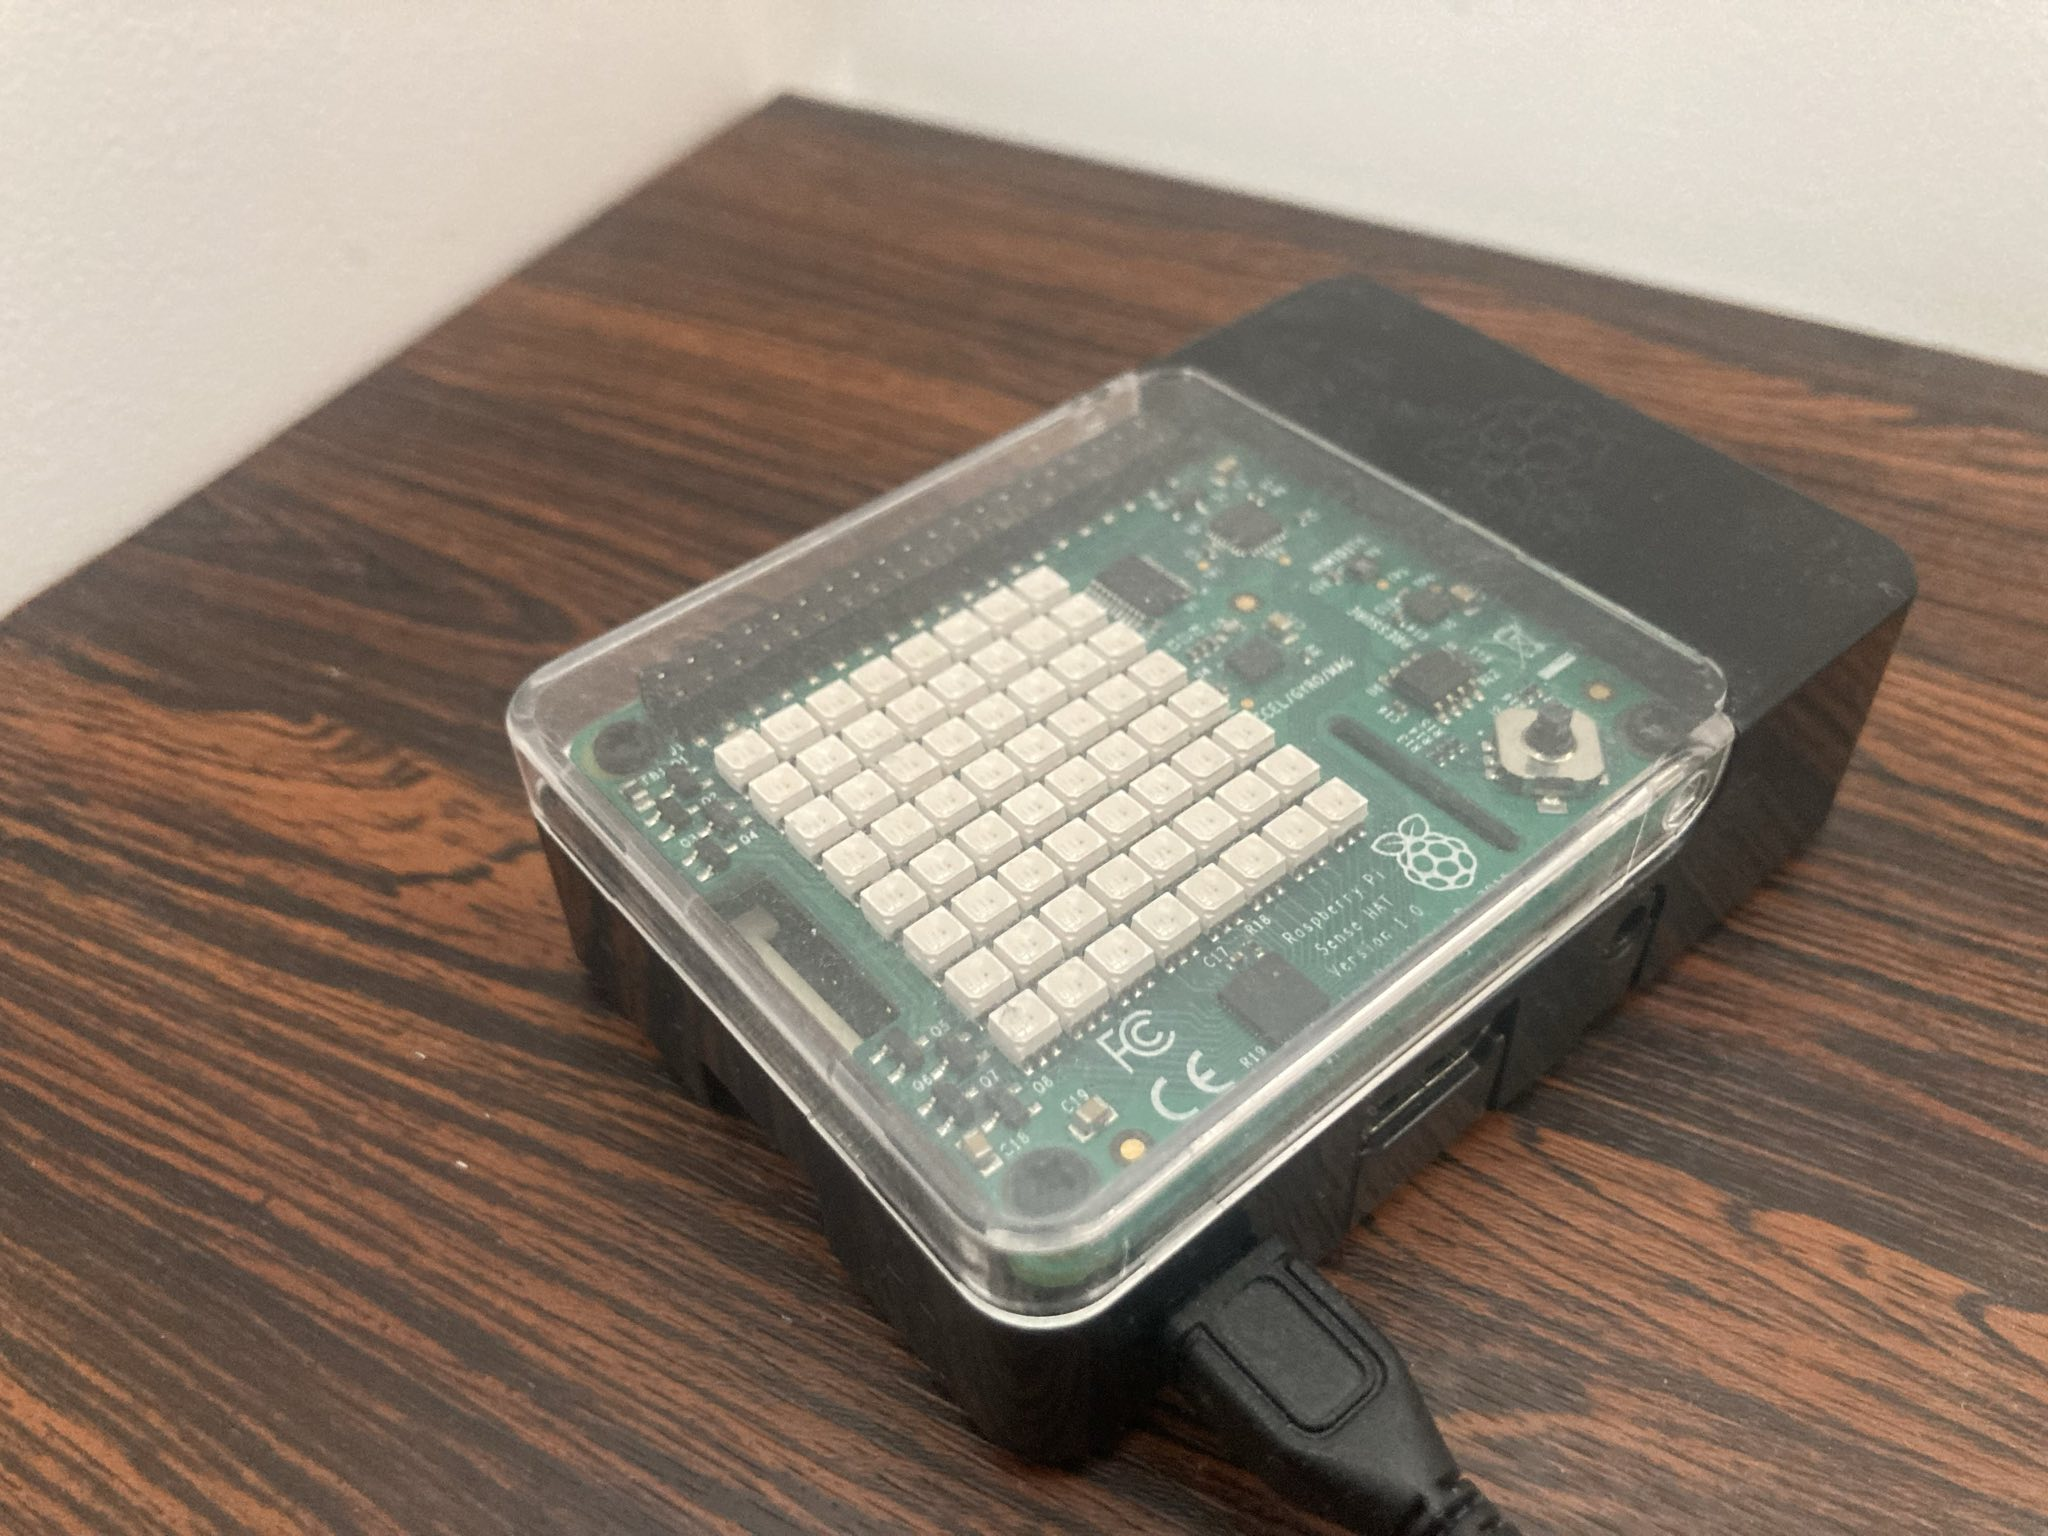
\includegraphics[width=0.8\linewidth]{figures/pi_3}
  \caption{Pi 3}
  \label{fig:pi3}
\end{subfigure}%
\begin{subfigure}{.5\textwidth}
  \centering
  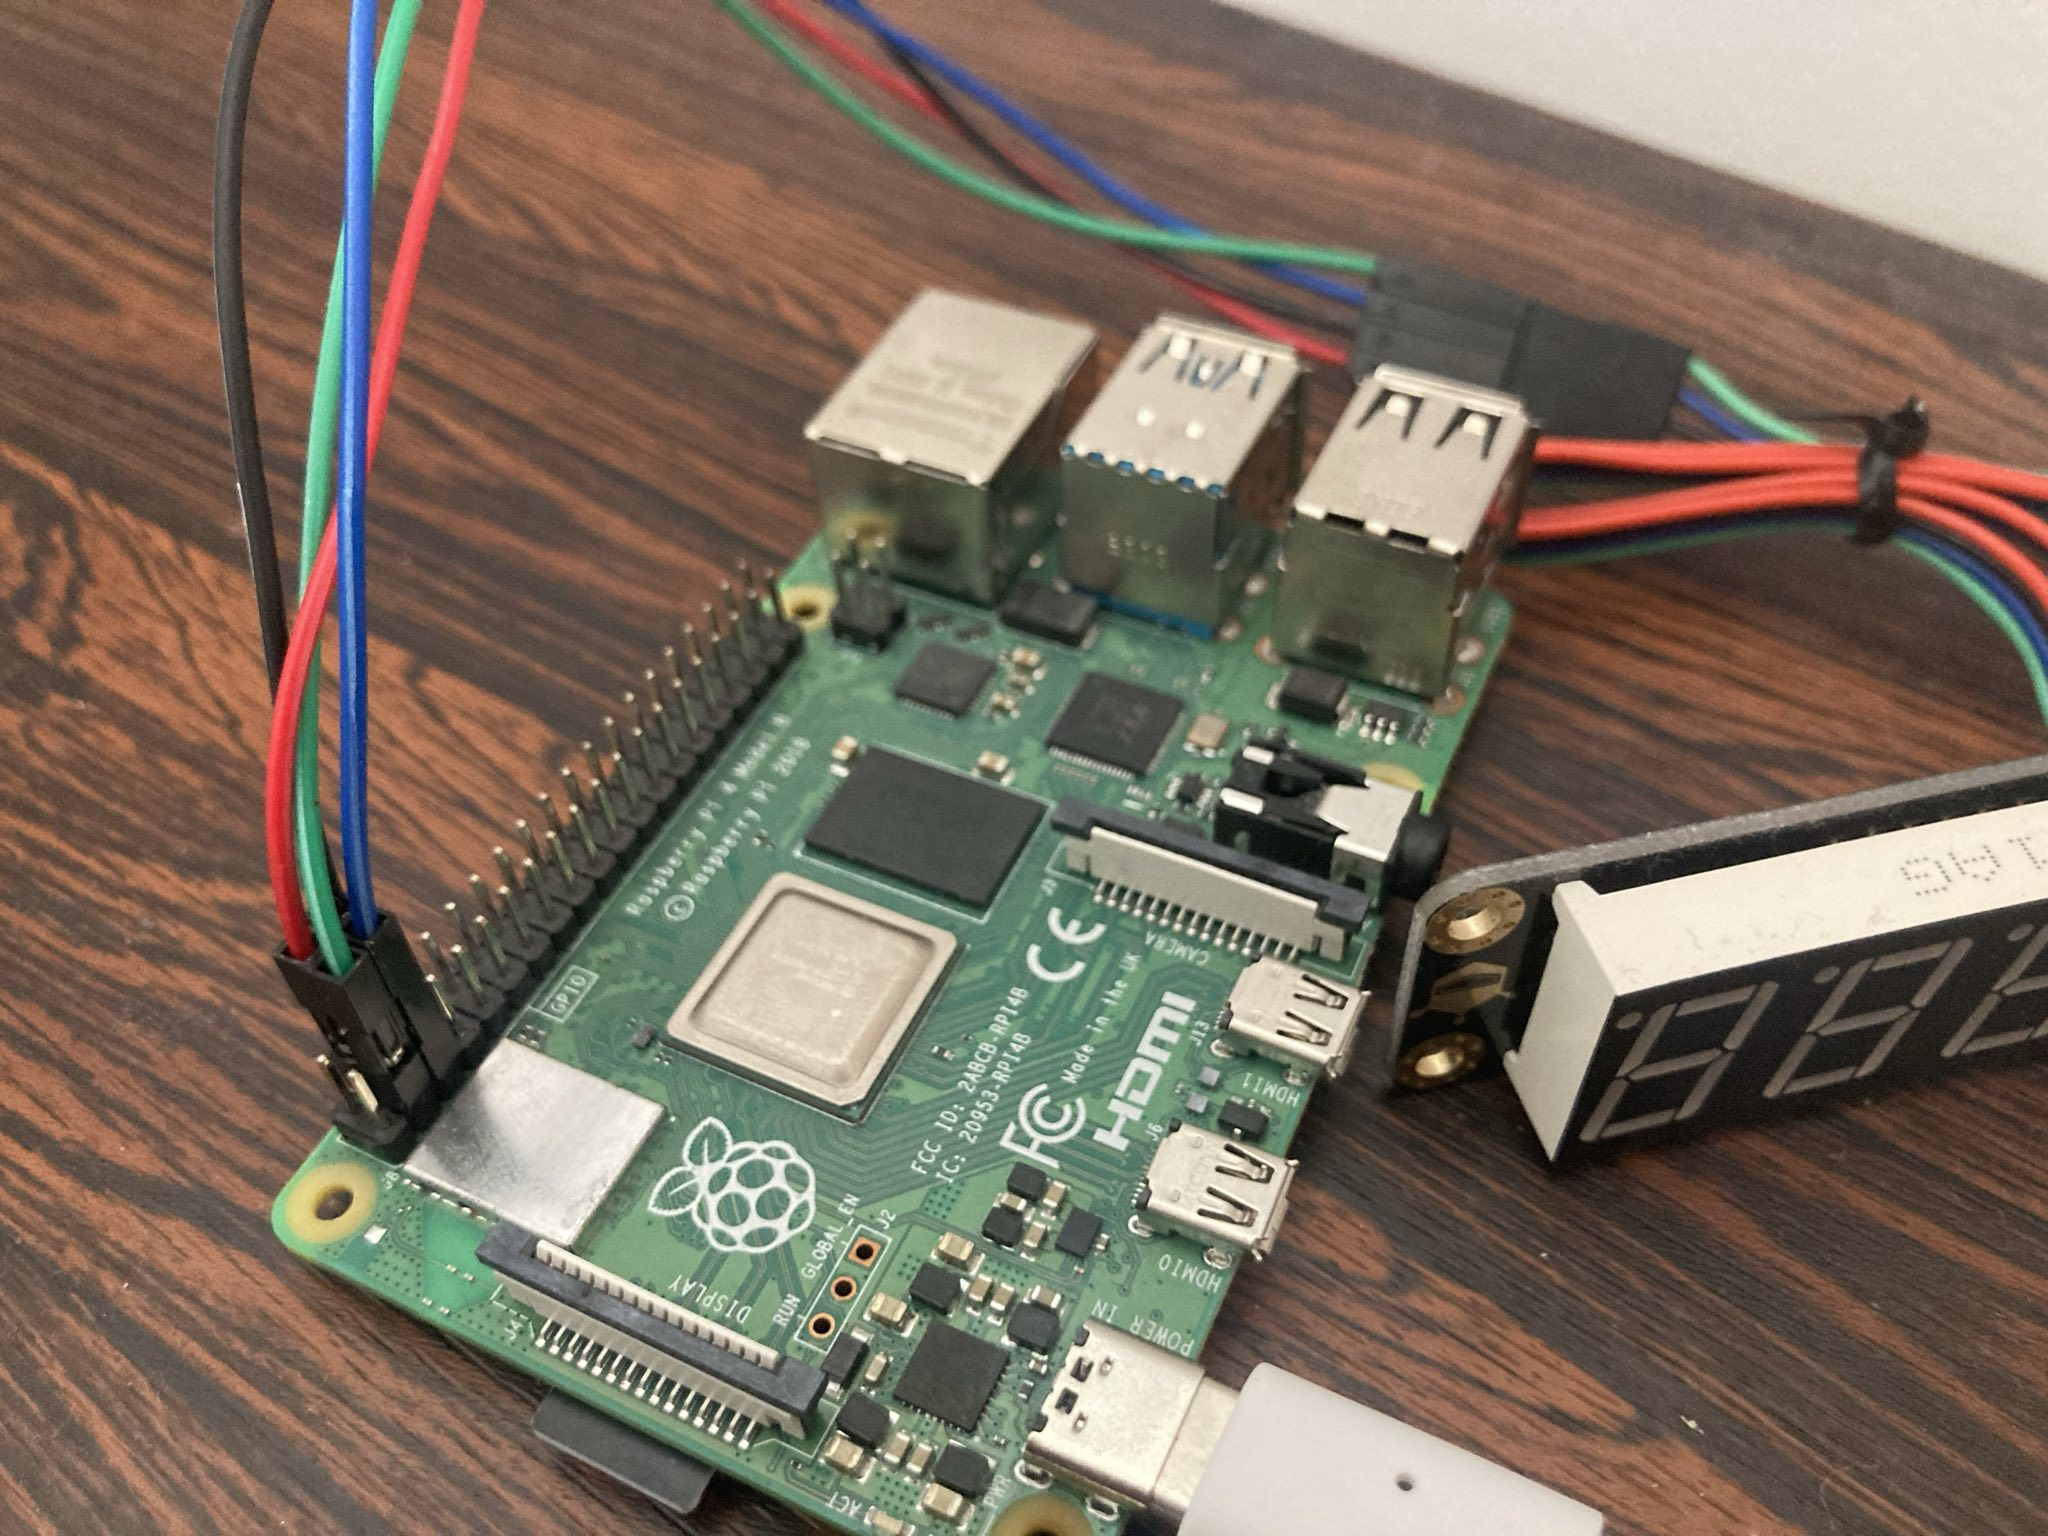
\includegraphics[width=0.8\linewidth]{figures/pi_4}
  \caption{Pi 4}
  \label{fig:pi4}
\end{subfigure}
\hfill
\begin{subfigure}{.5\textwidth}
  \centering
  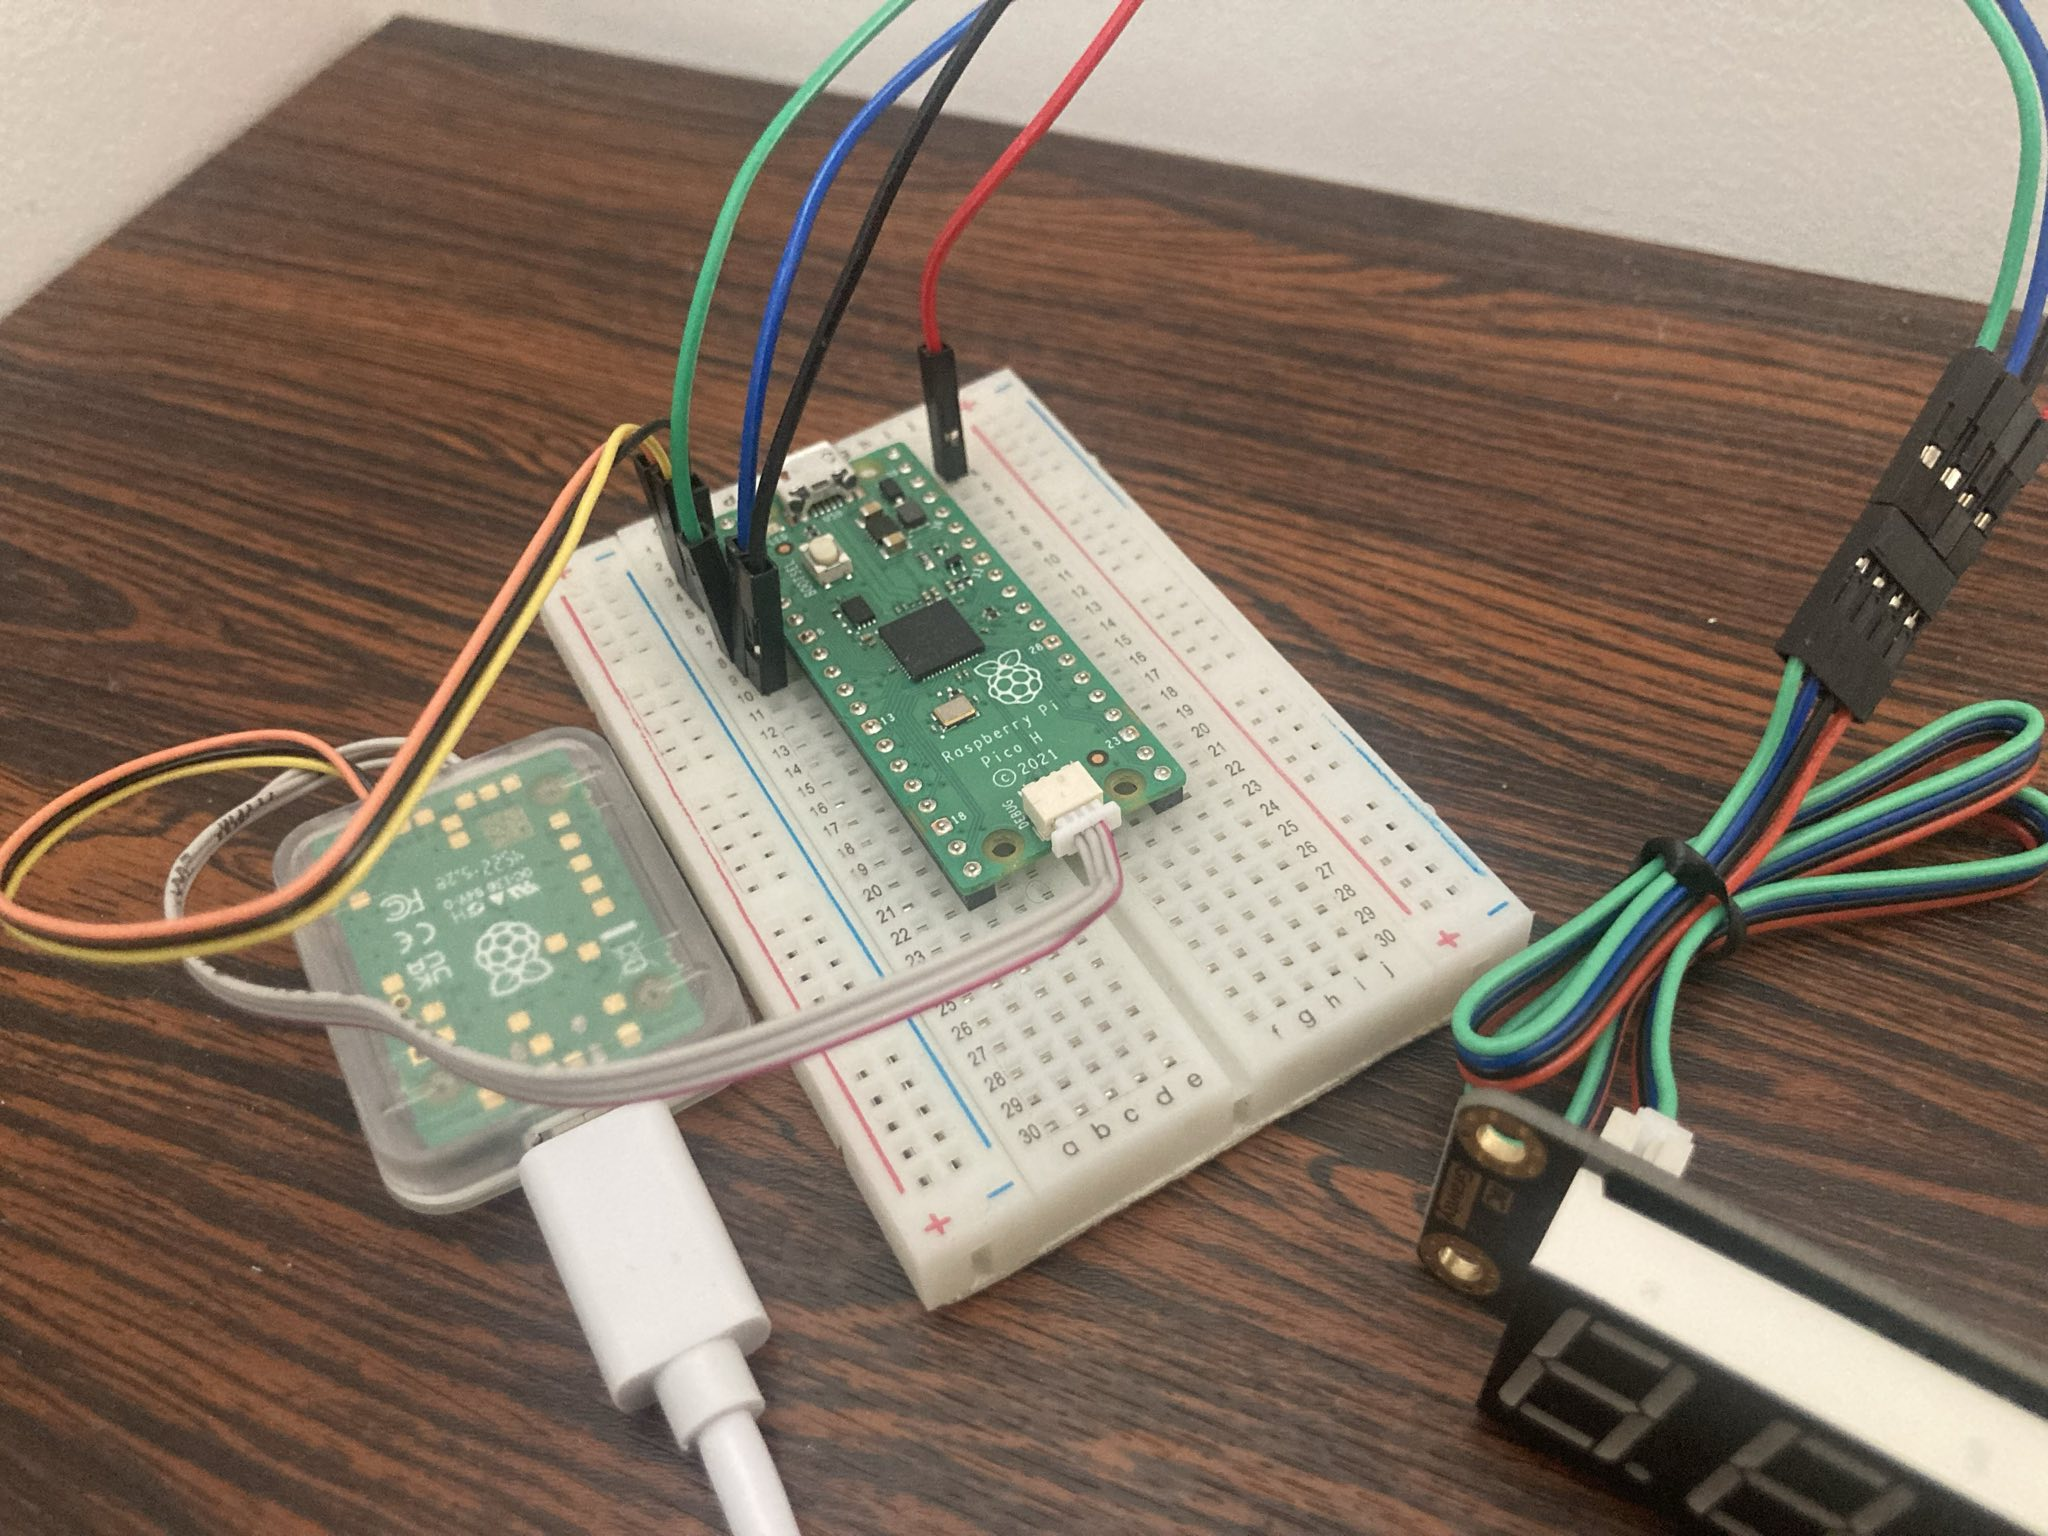
\includegraphics[width=0.8\linewidth]{figures/pi_pico}
  \caption{Pi Pico}
  \label{fig:pi_pico}
\end{subfigure}

\caption{Setups of....}
\end{figure}

\begin{table}[h]
	\centering
	\captionsetup{justification=centering}
	\begin{tabular}{l l}
		\toprule
        Connected device & Hardware \\ \midrule
        HTS221 sensor    & Raspberry Pi 3 Model B \\
        4-digit 7-segment display & Raspberry Pi 4 Model B \\
        4-digit 7-segment display & Raspberry Pi Pico \\
		\bottomrule
	\end{tabular}
    \caption{Concise overview of the setups}
	\label{tab:setups}
\end{table}


\section{Native development in Rust}
The Pi 4 can build the codebase, but the other two lack the capabilities for this, thus cross-compilation needs to be performed. Fortunately, Rust provides great support for this via the \texttt{target} flag. ARM64 can be targeted with \texttt{aarch64-unknown-linux-gnu}, and RP2040 with \texttt{thumbv6m-none-eabi}.

As the Pico is an MCU, it has some further requirements. First, it only supports \texttt{no\_std} build, see section~\ref{sec:runtimes}. Second, the memory layout also needs to be specified inside a file called \texttt{memory.x}.

To easily interface with the HTS221 sensor, the homonymous \texttt{hts221} Rust crate~\cite{gh:hts221} can be used. Unfortunately, for \texttt{embedded-hal} version 1 integration, a fork~\cite{gh:hts221-fork} had to be created. The \texttt{hts221} crate requires an I2C connection that follows the HAL specification, for this the \texttt{linux-embedded-hal} crate~\cite{gh:leh} is used.

For the implementation running on the Pi 4 we write the current local time. To establish the I2C connection the \texttt{rppal} crate~\cite{gh:rppal} is used. This library also follows the \texttt{embedded-hal} API, but is specifically tailored for Raspberry Pi devices. Due to the limited capabilities of the Pico, a simple incrementing counter is instead displayed. For the connection, the \texttt{rp-pico} crate~\cite{gh:rppico} is now utilized.  
% [Native driver development, hoe gaat het te werk en de grote verschillen voor native development voor een gewone Pi en een microcontroller zoals de Pi Pico.]
% Besides the implementation itself, two things are of significance to design a device driver in Rust. Namely, following the Embedded \gls{HAL} \gls{API}, see chapter~\ref{chap:hardware}, and supporting the desired target architecture.

\section{Embedded driver development in WebAssembly}
% [Om van native naar Wasm te gaan, wat moet er veranderen.]embedded-hal 0.2 vs 1.0 vermelden

To make the move from native to WebAssembly, everything related to the I2C connection itself is kept host-side. The device-specific logic, like reading the current temperature, is moved to the guest. Ideally, each implementation, conceptually, comes down to the schematic defined in Figure~\ref{fig:schematic}. But due to the myriad of differences between Wasmtime and WAMR, outlined in section~\ref{sec:runtimes}, no WebAssembly-specific code can be reused between them. This implementation, therefore, keeps everything each runtime interacts with inside two seperate directories.

\begin{figure}[ht]
    \centering
    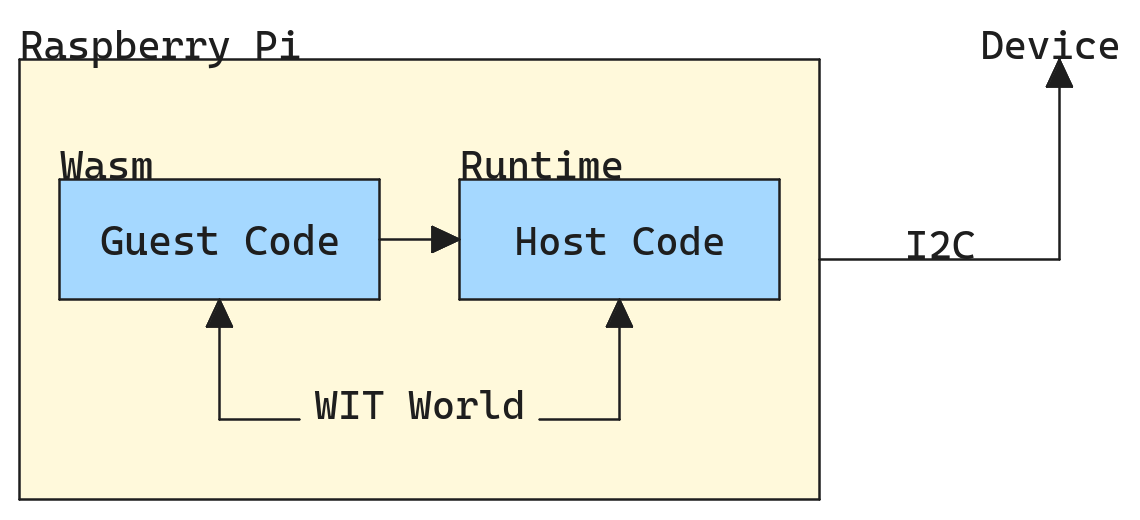
\includegraphics[width=0.5\textwidth]{figures/schema.png}
    \caption{Schematic overview of an implementation in WebAssembly.}
    \label{fig:schematic}
\end{figure}

\subsection{Schematic implementation for Wasmtime}

The Wasmtime implementation consists of three directories: \texttt{guest}, \texttt{host} and \texttt{wit}. The \texttt{wit} directory specifies two worlds, corresponding with the two devices being interacted with. This implementation thus contains two implementations that follow the schematic described by Figure~\ref{fig:schematic}.

% "we" vervangen door "deze masterproef, deze implementatie, deze oplossing"

\subsubsection{WIT world}

\begin{figure}[h]
\dirtree{%
.1 wit.
.2 device.wit.
.3 deps/i2c.
.3 deps.toml.
.3 deps.lock.
}
\caption{Structure of the \texttt{wit} subdirectory inside Wasmtime}
\label{fig:wit:dirtree}
\end{figure}

\begin{listing}[h!]

\begin{minted}[samepage]{rust}
world sensor {
    import wasi:i2c/i2c@0.2.0-draft;
    export hts: interface {
      use wasi:i2c/i2c@0.2.0-draft.{i2c, error-code};
      get-temperature: func(connection: i2c) -> result<string, error-code>;
      get-humidity: func(connection: i2c) -> result<string, error-code>;
    }
}

world screen {
    include wasi:i2c/imports@0.2.0-draft;
    export display: interface {
      use wasi:i2c/i2c@0.2.0-draft.{i2c};
      use wasi:i2c/delay@0.2.0-draft.{delay};
      write: func(connection: i2c, delay: delay, message: string);
    }
}
\end{minted}
\caption{The \gls{WIT} worlds to which guest and host bind.}
\label{code:wit}
\end{listing}

Both the guest components, as the Wasmtime host implementation, make use of the \gls{WIT} from codefragment~\ref{code:wit}, as stipulated in section~\ref{sec:guest} and corresponding with the \texttt{device.wit} from Figure~\ref{fig:wit:dirtree}. Herein, \texttt{wasi:i2c} is the proposal, see chapter~\ref{chap:architecture}. The display is represented by the \texttt{screen} world, which needs both \texttt{i2c} and \texttt{delay} from the proposal. The HTS221 is mapped with the \texttt{sensor} world, that only needs \texttt{i2c}. Therefore, the former just includes the imports from \texttt{wasi:i2c}, while the latter only imports \texttt{i2c}. The idea behind this WIT description is to keep it as generic as possible, this is why the \texttt{write} function accepts a string while the display only has four digits.

The \texttt{deps/i2c} contains the WIT interfaces from the proposal, both the \texttt{deps.lock} and \texttt{deps.toml} are files required for the correct workings of \texttt{wit-deps}.

\subsubsection{Guest code}

To reduce the size of the generated Wasm binaries, the guest implementations don't make use of Rust's std. For the generation of the guest components \texttt{cargo-component}, see section~\ref{sec:guest}, requires an adapter. Typicallly this adapter enables the usage of the std, but as the guest implementations doesn't make use of this an adapter is no longer needed. To solve this conundrum, an empty adapter is given to \texttt{cargo-component} via \texttt{empty.wasm} and \texttt{empty.wat}. Note that this uses \texttt{\#![feature(...)]}, which requires the usage of the nightly version of Rust.

It would be ideal if the \gls{Wasm} implementation of the sensor read would still use the \texttt{hts221} crate. For this, code needs to be supplemented to the generated bindings to make them compatible with the \texttt{embedded-hal} API. This supplementation is done via the \texttt{add\_i2c\_hal} macro inside the \texttt{wasi-embedded-hal} crate~\cite{gh:weh}.

\begin{listing}[h]
\begin{minted}[samepage]{rust}
#![no_std]
#![no_main]
mod bindings;

// To make the generated bindings compatible with the `embedded-hal` API
add_i2c_hal!(i2c);

struct Component {}

impl Guest for Component {
  // Omitting implementations of the exports inside of the binded world
}

// Omitting the definition of a global alllocater and a panic handler,
//  needed by Rust because of `no_std`.

bindings::export!(Component with_types_in bindings);
\end{minted}
\caption{Stripped down version of a guest component for Wasmtime.}
\label{code:guest}
\end{listing}

Codefragment~\ref{code:guest} describes how, conceptually, each component implementation looks like.

\subsubsection{Host code}

\begin{figure}[h]
\begin{subfigure}{.5\textwidth}
  \dirtree{%
  .1 host.
  .2 src.
  .3 device.rs.
  .3 display.rs.
  .3 sensor.rs.
  }
\end{subfigure}%
\begin{subfigure}{.5\textwidth}
    \centering
    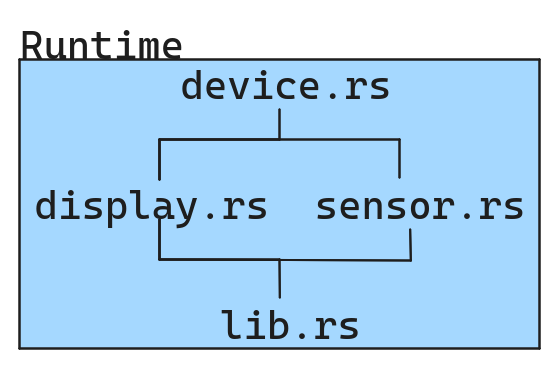
\includegraphics[width=0.5\textwidth]{figures/host.png}
\end{subfigure}
\caption{Structure of the Wasmtime host directoy structure vis-à-vis with its logical structure.}
\label{fig:host}
\end{figure}

The WIT interface imports (parts of) the \texttt{wasi:i2c} interfaces. Therefore, it is not possible to run components via the \texttt{wasmtime} command line, explained in section~\ref{sec:host}, and a custom host is necessary. The most basic version of this custom host would simply be a standalone implementation of each world. Every world implementation then has their own fulfillment of the imports, resulting in lots of code redudancy. Therefore, a more involved host implementation, like the structure defined in Figure~\ref{fig:host}, is more practical. Here, the world implementations can share their usage of \texttt{device.rs} for the fulfillment of the imports via the \texttt{with} keyword, as demonstrated inside codefragment~\ref{code:with}. It is important that these paths be fully qualified. Otherwise errors will be thrown by the Rust compiler. 

Each world implementation in itself is a module that splits the standard procedure, see~\ref{sec:runtimes}, for executing a method from a \gls{Wasm} binary in two functions:

\begin{enumerate}
  \item \texttt{new}: Responsible for adding the implemented i2c and delay structs from device to the linker, creation of the host state and populating it, creation of the store and instantiation of the bindings. 
  \item \texttt{run}: Executes a certain function from the component. The parameters are hardcoded.
\end{enumerate}

The purpose of this deviation from the standard procedure is twofold. First, it allows calling the exported function without the need to instantiate the component each time. Second, it provides a shared function signature for running a component.

\begin{listing}[h]
\begin{minted}[samepage]{rust}
// device.rs
bindgen!({
    path: "../wit/deps/i2c",
    world: "wasi:i2c/imports",
    with: {
        "wasi:i2c/i2c/i2c": device::I2c,
        "wasi:i2c/delay/delay": device::Delay,
    }
});
// display.rs
bindgen!({
    path: "../wit",
    world: "screen",
    with: {
        "wasi:i2c/i2c/i2c": device::I2c,
        "wasi:i2c/delay/delay": device::Delay,
    }
});
\end{minted}
\caption{Usage of the \texttt{with} keyword inside the \texttt{bindgen}'s of \texttt{device.rs} and \texttt{display.rs}.}
\label{code:with}
\end{listing}

\subsection{Schematic implementation for WAMR}

This implementation represents the schematic from Figure~\ref{fig:schematic} for WAMR, hower there's no support for preview two. This aplication, thus, cannot make use of \gls{WIT}, nor pass a proper I2C connection to the guest because there's no notion of a WIT resource. Therefore, the connection is now kept global. In Rust, there's no default way to keep a variable global, but for this implementation the \texttt{once\_cell}~\cite{gh:once-cell} crate is used. 

All guest-to-host and host-to-guest communication is considered unsafe on a memory-safety basis, this is because WAMR is written in C, a language infamous for how unsafe it is. Furthermore, the WAMR Rust SDK mandates that imports and exports are called and developed as extern C functions. This leads to a module implementation conceptualized by codefragment~\ref{code:wamr:guest}. The host cannot directly bind with the resulting binary, instead it has to register the import and find the exports. 
For passing parameters to the exports, a vector of \texttt{WasmValue}s is passed. A \texttt{WasmValue} can be a void, 32-bit signed integer, 64-bit signed integer, 32-bit float, 64-bit float or a 128-bit signed integer. Each value is underlying stored as an array of 32-bit unsigned integers. The exported \texttt{setup}function can then be called with an array containing a \texttt{WasmValue::Void}, for \texttt{write} a vector of four \texttt{WasmValue::I32}'s are passed.

\begin{listing}[h]
\begin{minted}[samepage]{rust}
#![no_std]
#![no_main]

#[link(wasm_import_module = "host")]
extern "C" {
    // The term _slave_ is still used because `rppal` still uses this.
    fn host_i2c_write(slave_address: u16, data: u8);
}

#[export_name = "setup"]
pub fn setup() { /* Omitting definition */ }
#[export_name = "write"]
pub fn write(d0: i32, d1: i32, d2: i32, d3: i32) { /* Omitting definition */ }

// Omitting the definition of a global alllocater and a panic handler,
//  needed by Rust because of `no_std`.
\end{minted}
\caption{Stripped down version of a guest module for WAMR.}
\label{code:wamr:guest}
\end{listing}

% Host uitleggen
%   - Functies moeten gevonden worden, host_i2c_write moet geregistered worden
%   - Paramters zijn basic van type, hierdoor geven we het door als i32
%   - Bij nieuwe instance moet de stack size mee gegeven worden

% [vertellen dat ik in WAMR constrained was tot het doorgeven van simpele datatypes en dan maar met die globale connectie gewerkt heb]
% As there's no support for preview two, it is not possible to make use of \gls{WIT}, nor pass a proper I2C connection to the guest [omdat we geen resources kunnen doorgeven]. Therefore, instead of passing the connection, it is now kept global inside the host. Furthermore, instead of passing a string as an argument to the \texttt{write} function, each byte of the string is mapped to a 32-bit integer and seperately given as an argument.

On the Raspberry Pi Pico, there's no filesystem, thus no capability of reading the \gls{Wasm} binary from disk. Instead, a \texttt{hexdump} can be taken from the binary, and then these bytes can be hardcoded as a vector of unsigned 8-bit integers inside the host. 

Under the hood, Rust uses \texttt{rust-lld} for the cross-compilation to the Pico~\cite{lld}, but WAMR uses the \path{arm-none-eabi-gcc} linker. This results in a CMAKE error when building the SDK~\cite{gh:wrs:error}, and thus disabling cross-compilation.

% To resolve this issue, a \texttt{hexdump} needs to be taken from the binary, and then these bytes need to be hardcoded as a vector inside the host. Under the hood, Rust uses \texttt{rust-lld} for the cross-compilation to the Pico~\cite{lld}, but WAMR uses the \texttt{arm-none-eabi-gcc} linker. This results in a CMAKE error when building the SDK~\cite{gh:wrs:error}.

